\section{Introduction}

Policies that generalize are trained on volumes of data no single lab records by hand. $\pi_0$ pretrains on more than 10,000 hours of robot data~\cite{pi0}; LingBot-VLA on about 20,000 hours from nine dual-arm platforms, with success rates still rising at that scale~\cite{lingbotvla}; EgoScale on 20,854 hours of egocentric human video, where action-prediction loss falls log-linearly with hours and that loss tracks success on a real robot~\cite{egoscale}. The last result is the one that matters here, because it makes egocentric human video rather than teleoperation the scalable source: a person wearing a camera while doing chores is training data. What the hours contain matters as much as how many there are. Lin et al.~\cite{lin2025scaling} collected 40,000 demonstrations and found that a single-task policy's generalization follows a power law in the number of training environments and objects, that additional demonstrations in the same environment stop helping past a threshold, and that 32 environments with one object each were enough for 90\% success in rooms and on objects never seen. The useful unit of data is a new combination of surface, object, lighting and clutter around the same action. We call that combination the ontology of a scene, and diversity of ontology, not hours, is what a policy needs.

\begin{figure}[t]
\centering
\begin{subfigure}{0.33\linewidth}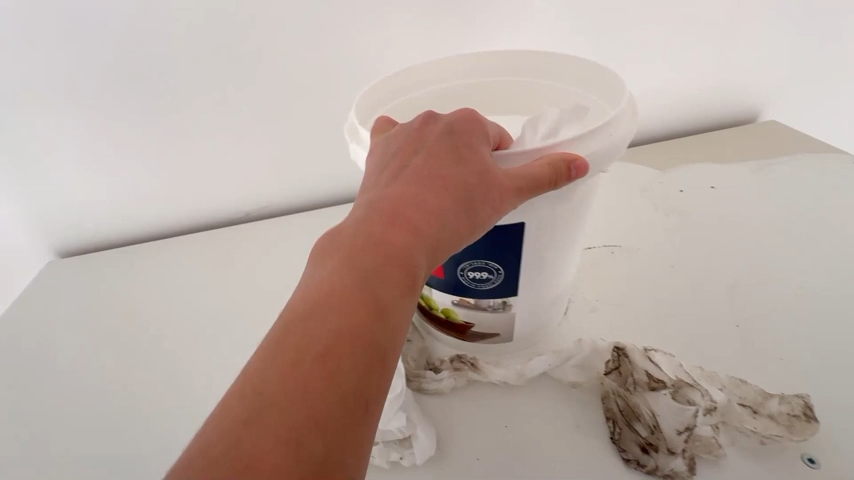
\includegraphics[width=\linewidth]{s03_original.png}\caption{what we started with}\end{subfigure}\hspace{2mm}
\begin{subfigure}{0.33\linewidth}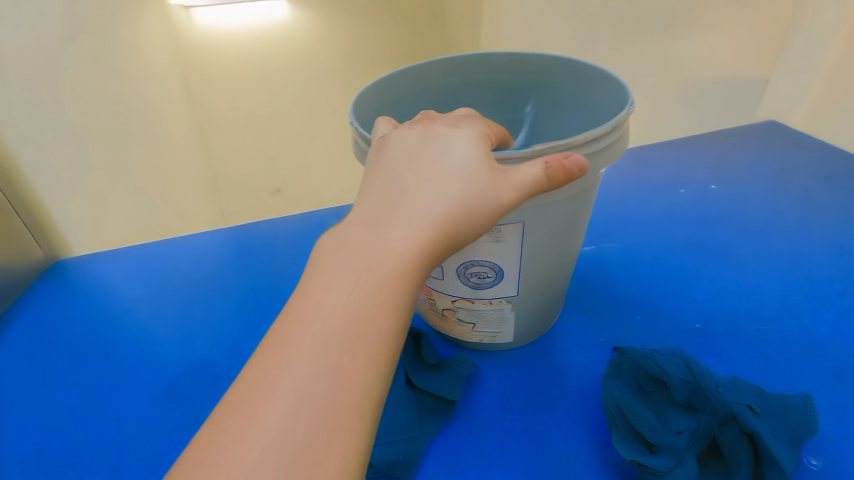
\includegraphics[width=\linewidth]{s04_created.png}\caption{what we created}\end{subfigure}
\caption{The running example. (a) A real clip: a person wiping a counter with a bucket and paper towels. (b) The variant rendered when asked to change only the countertop to blue. Counter color, hand pose, bucket geometry and motion are as intended; the beige wall, blue towels and bucket, and new ceiling light were not asked for.}
\label{fig:teaser}
\end{figure}

Recording that diversity is where the cost sits. An hour of egocentric video costs 8 to 15 USD in collector pay \verify{source for the hourly rate}, so 20,000 hours for a single task is 160,000 to 300,000 USD before anyone has found that many different kitchens, and the kitchens are the hard part: the scaling result says the next hour in the same room is close to worthless. The existing shortcuts each give up something. MimicGen multiplies 200 human demonstrations into 50,000 by replaying trajectory segments in new object poses, but in simulation and for robot trajectories, not video~\cite{mimicgen}. FieldGen automates the reaching phase of a demonstration and keeps the human for contact~\cite{fieldgen}; it saves operator time, not environments. Domain randomization perturbs colors and textures with no notion of the task, so a cleaning bucket gets a texture no bucket has~\cite{tobin2017}. Generative augmentation with image diffusion models produces plausible single frames but does not hold hands and objects steady across a clip~\cite{rosie,genaug}. Structure-conditioned video models can restyle a whole clip~\cite{gen1,controlnet}, and NVIDIA's Cosmos family packages this for physical AI~\cite{cosmos2025}, but none of them decides what in a clip should change and what must stay fixed.

We take the clip as the unit and permute the ontology around the recorded action. A reasoning model reads the clip and writes the scene as a structured ontology: the task, each object with its role in that task, and the variations each object could plausibly take while the task stays the same. A language model filters the candidates and writes a prompt, a segmenter builds a mask of the one surface to change, and a guided video-to-video model renders the variant with the hand motion intact (Fig.~\ref{fig:teaser}). On 116 clips from 8 recordings the reasoning stage admits 72 variations per clip, so a 15-second clip becomes 18 minutes of candidate video and a 10-minute recording about 4 hours, a 72-fold multiplier with no new recording and no new kitchen. The same arithmetic sets the limit: a render costs 20 minutes on one A100, or 80 GPU-hours per synthetic hour, so at today's speed the pipeline buys diversity rather than cheaper hours. For a robotics company the value is in the loop this closes. Real recordings from a deployment become synthetic variants the same day, the variants retrain the policy, the retrained policy goes back on the robot, and its new recordings seed the next round; the pipeline turns the real-to-sim-to-real cycle from a collection campaign into a batch job. The paper reports what the pipeline produces and where it stops. Single-surface recolors keep hand pose, object shape and motion, but the edit does not stay inside its mask: in the counter-wiping clip the protected region shifts by a mean CIE76 $\Delta E$ of 35 against 75 for the target. Scenes with many textures recolor wholesale, and two attempts at action-level change with Cosmos Predict2 returned the scene unchanged. Whether appearance diversity alone makes a policy more general, or whether action generation has to be solved first, is the question these results leave open.
